\subsection{Quantitative Evaluation}\label{sec:quality}
In this part, we quantitatively evaluate our proposals on the three trajectory datasets in terms of both visual quality and efficiency.

\begin{figure*}[t]
	\centering
	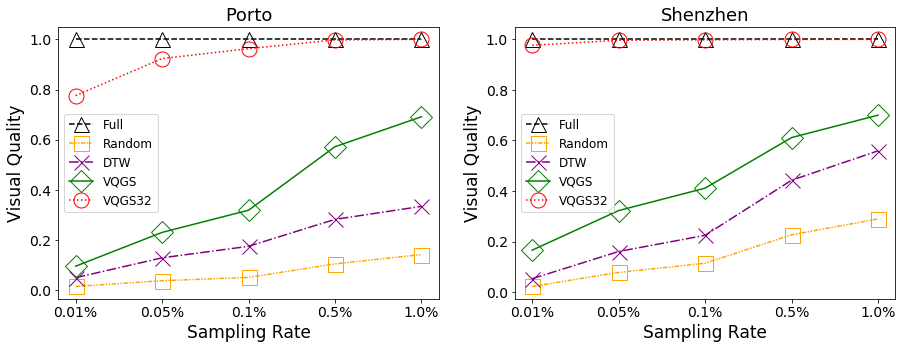
\includegraphics[width=0.9\textwidth]{pictures/quantitative_study_icde/rate_quality.png}
	%\vspace{-3mm}
	\caption{Visual quality vs. sampling rates(T1).}
	\label{fig:sample_quality}
	%\vspace{-3mm}
\end{figure*}

\begin{figure*}[t]
	\centering
	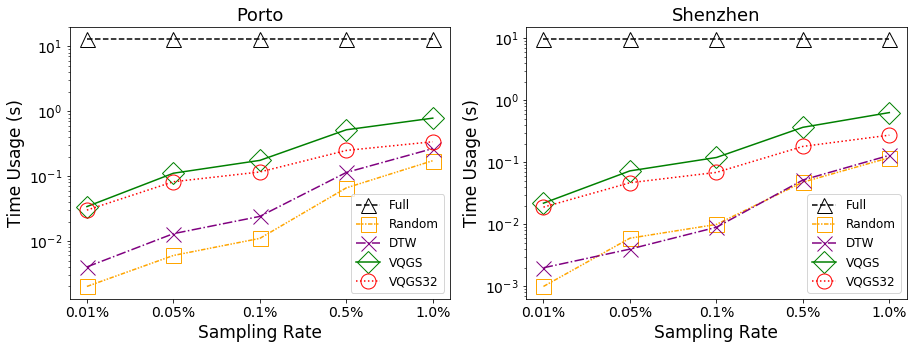
\includegraphics[width=0.9\textwidth]{pictures/quantitative_study_icde/rate_rendertime.png}
	%\vspace{-3mm}
	\caption{Processing time vs. sampling rates.}
	\label{fig:rate_quality}
	%\vspace{-3mm}
\end{figure*}


\begin{figure*}[t]
	\centering
	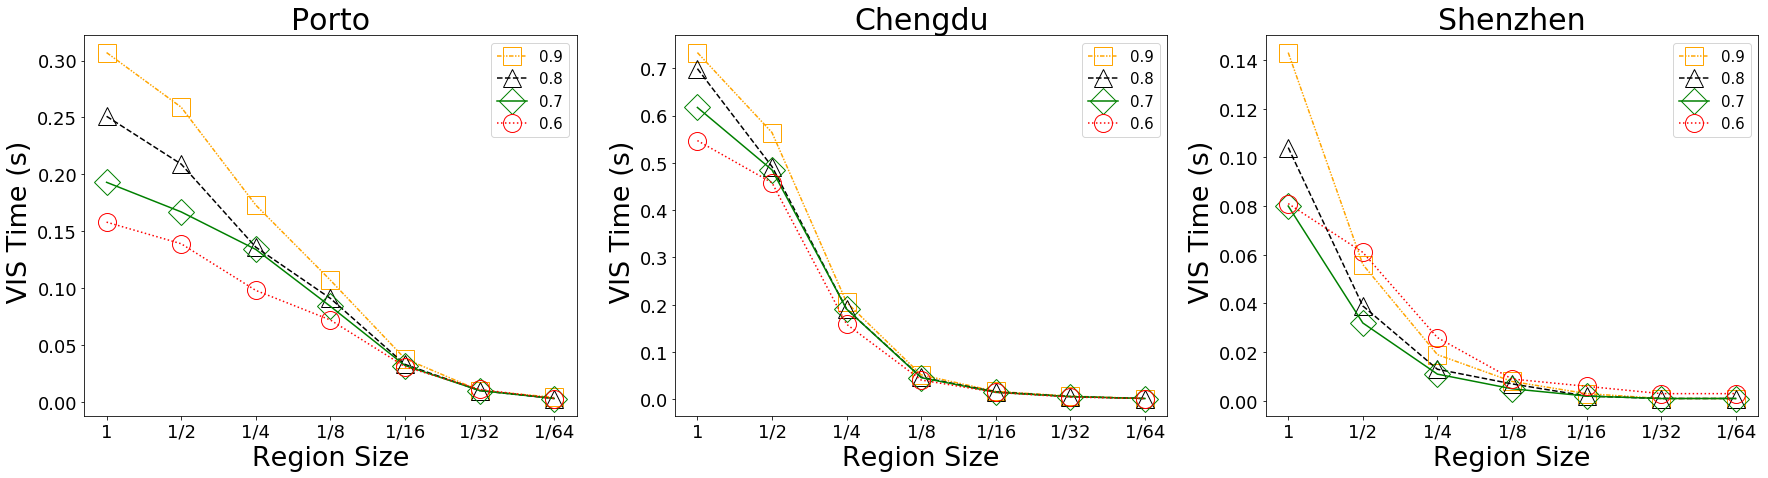
\includegraphics[width=0.9\textwidth]{pictures/quantitative_study_icde/size_rendertime.png}
	%\vspace{-3mm}
	\caption{Response time vs. region size.}
	\label{fig:size_rendertime}
	%\vspace{-3mm}
\end{figure*}



\begin{figure*}[t]
	\centering
	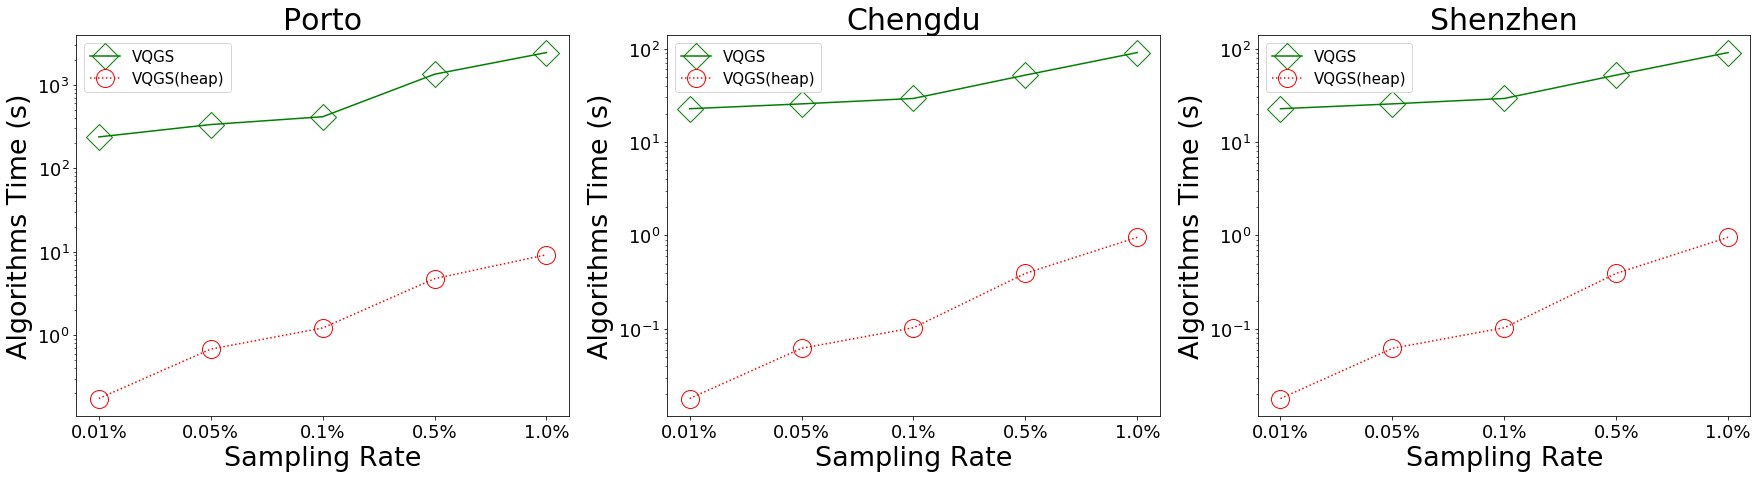
\includegraphics[width=0.9\textwidth]{pictures/quantitative_study_icde/rate_algtime.png}
	%\vspace{-3mm}
	\caption{Algorithm running time vs. sampling rate.}
	\label{fig:rate_algtime}
	%\vspace{-3mm}
\end{figure*}
%\begin{figure}[t]
%	\centering
%	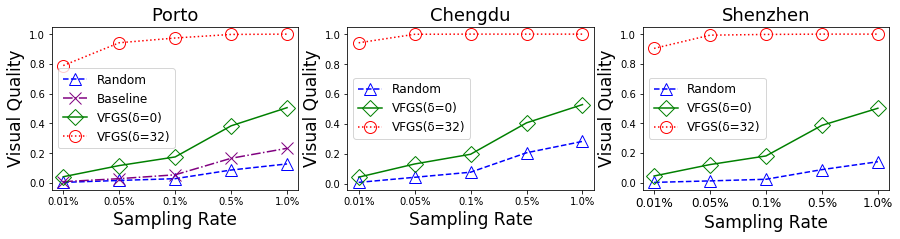
\includegraphics[width=0.5\textwidth]{pictures/quantitative_study_icde/sample_quality.png}
%	\vspace{-8mm}
%	\caption{Visual quality vs. sampling rates.}
%	\label{fig:sample_quality}
%	\vspace{-3mm}
%\end{figure}

%\begin{figure}[t]
%	\centering
%	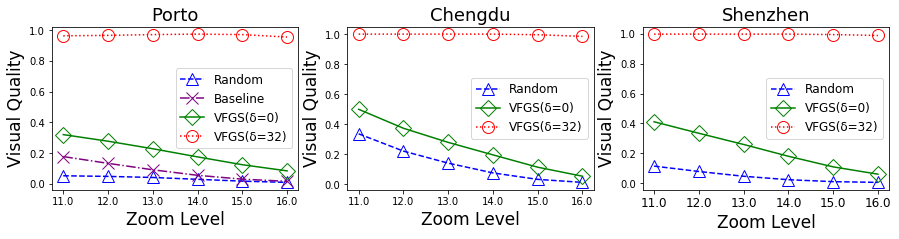
\includegraphics[width=0.5\textwidth]{pictures/quantitative_study_icde/zoom_quality.png}
%	\vspace{-8mm}
%	\caption{Visual quality vs. zoom level.}
%	\label{fig:zoom_quality}
%	\vspace{-3mm}
%\end{figure}

\stitle{Visual quality} Figure~\ref{fig:sample_quality} reports the visualization quality (as defined in Equation~\eqref{eqref:loss}) of the methods under different sampling rate. We consider the entire region in each dataset for this experiment. The results show that both $\vats$ and $\vatss$ achieve significantly high quality than $\rand$ and $\mathsf{DTW}$ under the same sampling rate. This is because $\vats$ and $\vatss$ explicitly considers visual quality in the sampling process. Specifically, $\vatss$ has a quality close to 1 with a sampling rate less than 1\%. $\mathsf{DTW}$ has a higher quality than $\rand$ because it considers the diversity of trajectories. 

In Figure~\ref{fig:sample_quality}, we report the visualization time (i.e., the time to generate visualization using the sampled trajectories) for the methods under different sampling rates. We still consider the entire region in this experiment and the visualization time of $\full$ is included at the top of each figure for reference. The results show that all sampling methods achieve significantly shorter visualization time than $\full$, which confirms our observation that sampling is effective in improving visualization efficiency. Under the same sampling rate, $\vats$ and $\vatss$ take longer visualization time than $\rand$ and $\mathsf{DTW}$ because $\vats$ and $\vatss$ are more likely to select long trajectories for quality maximization. Combining Figure~\ref{fig:sample_quality} and~\ref{fig:sample_quality}, we can conclude that $\vatss$ can achieve high visualization quality with  short visualization time.   

We also eventuate the \textit{response time} of the $\avats$ framework under different quality guarantee and region size in Figure~\ref{fig:size_rendertime}. The response time is defined as the time taken to process the user query region to generate the visualization result. We contain the regions to be rectangles with a constant height/width ratio and measures the size of a region by dividing its height over the height of the entire region. Under each region size, we report the average response time of three typical regions, i.e., a dense region, a sparse region and a medium region. The results show that $\avats$ achieves a short response time (less than 1 second in all cases) for different region size and quality guarantees. The response time decreases rapidly when the region size shrinks as there are fewer trajectories in a smaller region. The response time required to achieve a high quality (e.g., 0.9) is not significantly longer than a low quality (e.g., 0.6) as quality improves quickly with the number of sampled trajectories. 

In Figure~\ref{fig:rate_algtime}, we report the running time of $\vatss$ with and without heap-based lazy computation under different sampling rate. The results show that the heap-based optimizations reduces the running time of $\vatss$ by 2-3 orders of magnitude. For the sampling rates we considered, $\vatss$ runs efficiently and can finish within 1 second for the entire dataset.                                  

 



%\stitle{Running time evaluation}

%\begin{figure}[t]
%	\centering
%	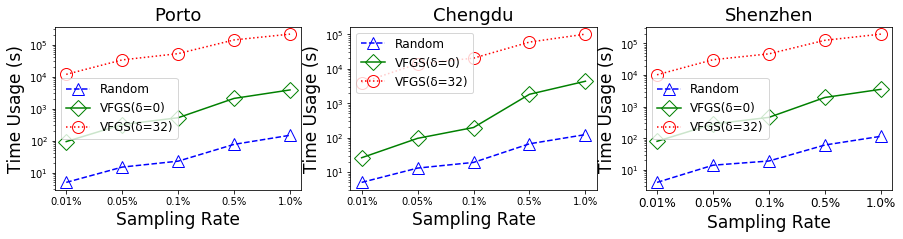
\includegraphics[width=0.5\textwidth]{pictures/quantitative_study_icde/sample_time.png}
%	\vspace{-8mm}
%	\caption{Time usage vs. sampling rates.}
%	\label{fig:sample_time}
%	\vspace{-3mm}
%\end{figure}

%\begin{figure}
%	\centering
%	\small
%	\begin{tabular}{cc}
%		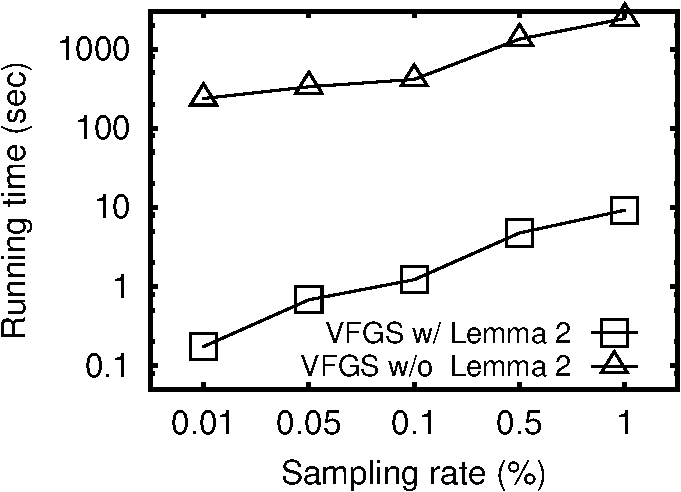
\includegraphics[width=0.44\columnwidth]{pictures/tporto}
%		&
%		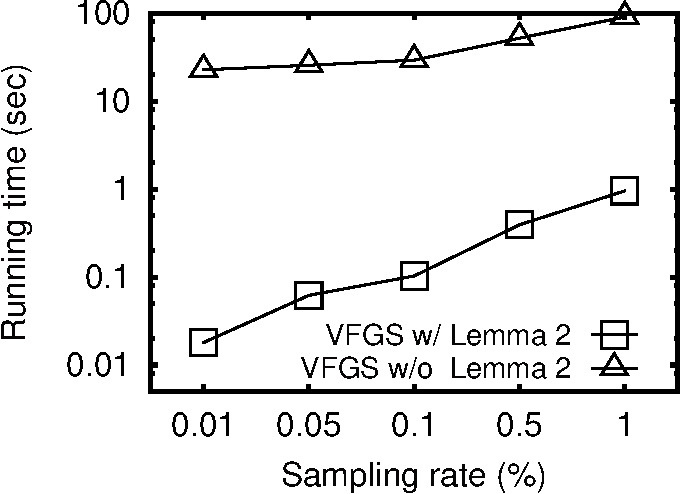
\includegraphics[width=0.44\columnwidth]{pictures/tshenzhen}
%		\\
%		(A) \pt{}
%		&
%		(B) \sz{}	
%	\end{tabular}
%	\vspace{-3mm}
%	\caption{Running time of $\vats$ w/ and w/o Lemma~\ref{lem:submodular}.}
%	\label{fig:cost}
%	\vspace{-6mm}
%\end{figure}
%\QM{unfininshed}
%We first conduct an experiment to evaluate the rendering cost by datasize. We vary the number of trajectories from 1000 to 1 million, which are randomly selected from \pt{} dataset. The experimental results are summarized in Table~\ref{tab:gpu}. We observe that the rendering cost is linear with the input data trajectories.
%
%We first report the running time of our $\vats$ algorithm in Figure~\ref{fig:cost} by varying the sampling rate from $0.01\%$ to $1\%$. The results show that $\vats$ is quite slow without the submodularity of contribution value, which agrees with Lemma~\ref{lem:submodular} in Section~\ref{sec:opt}.
%Then we shown the total time usage with sampling rate as Figure~\ref{fig:sample_time}. {*******}
%
%The optimized $\vats$ (e.g., $\vats$ with Lemma~\ref{lem:submodular}) outperforms $\vats$ by one to three orders of magnitudes on both datasets. The result show that running time of our $\vats$ algorithm is below 1 second in most cases. We have shown that $\vats$ provides good visualization performance with a low sampling rate (e.g., $0.1\%$ or $1\%$) in Section 6.1 and 6.2,  and Table~\ref{tab:gpu} suggests that the rendering latency scales almost linearly with dataset cardinality. By significantly reducing the dataset cardinality with sampling, $\vats$ can effectively reduces the rendering latency to make interactive visualization possible without sacrificing visual quality. For example, rendering the full $\pt{}$ dataset takes about \QM{34 seconds}, with a sampling rate of $1\%$, $\vats$ can bring down the rendering latency to less than 1 second.

\begin{table}
	\centering
	\small
	\caption{Visualization rendering cost}
	\begin{tabular}{|c|c|c|c|c|} \hline
		No. Trajs & GPS points & Mapping (s) & Rendering (s) & Total (s)\\ \hline
		1,000& 31,300 & 0.027 & 0.003 & 0.03 \\ \hline
		10,000& 31,6531 & 0.169 & 0.005 & 0.174\\ \hline
		100,000& 316,7120 & 1.701 & 0.057 & 1.758 \\ \hline
		1,000,000& 31,646,379 & 15.562 & 0.592 & 16.154 \\ \hline
	\end{tabular}	\label{tab:gpu}
\end{table}
